\chapter{Popis navržených řešení}

V předešlé kapitole byla vysvětlena základní problematika, která souvisí s virtualizací síťových funkcí, cloud computingem a softwarově definovanými sítěmi. Zároveň byla popsána referenční architektura frameworku pro virtualizaci síťových funkcí. Tato kapitola bude již věnována konkrétnímu příkladu využití virtuálních síťových funkcí v cloudovém prostředí. Nejprve zde popsána navržená architektura pro privátní cloudovou platformu využívající virtualizaci síťových funkcí, kterou mohou využívat všichni její uživatelé. Pro tuto cloudovou platformu a pro její uživatele byli navrženy dva příklady virtuálních síťových funkcí. U obou příkladů jsou uvedeny scénáře a způsob jakým jsou navrženy.

\section{Požadavky na VNF řešení}



\begin{itemize}
\item Univerzálnost - Celé řešení musí být postavené tak, aby ho mohli využívat všichni uživatelé dané cloudové platformy. 
\item Jednoduchost - 
\item Otevřenost a Flexibilita - 
\item Kompatibilita se stávající síťovými prvky - 
\end{itemize}

\section{Architektura navrženého řešení}

Architektura navrženého řešení byla implementována pomocí cloudové platformy OpenStack a SDN řešení OpenContrail. Obrázku č. \ref{fig:VNF_overview} znázorňuje tyto technologie v souvislosti s referenční architekturou popsanou v kapitole \ref{sub:architektura}. Je nutné říci, že obě technologie nezapadají přímo do jedné z částí referenční architektury. Naopak v některých případech se překrývají nebo se v ní doplňují.

\begin{figure}[h]
\begin{centering}
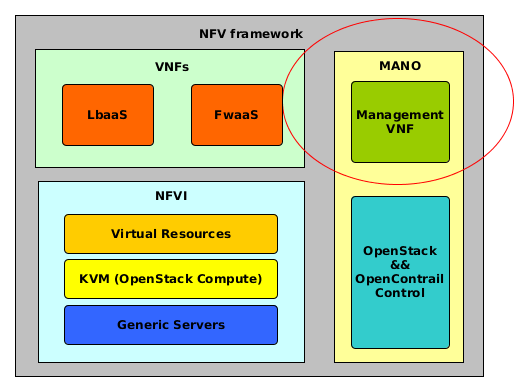
\includegraphics[scale=0.51]{images/VNF_overview}
\par\end{centering}
\caption{Architektura NFV řešení\label{fig:VNF_overview}}
\end{figure}

OpenStack byl zvolen, protože se jedná o největší open-source cloudovou platformu na světě. OpenStack tvoří část správy infrastruktury. Hardwarová vrstva infrastruktury se může skládat z libovolných serverů, na kterých je nainstalován KVM hypervizor. Tento hypervizor tvoří virtuální vrsvu a byl vybrán, protože je nejčastěji používán společně s OpenStackem. Avšak v případě potřeby by zde mohl být použit i jiný hypervizor, pokud bude zachována kompatibilita vůči OpenStacku.

OpenStack spravuje převážně zdroje týkající se výpočeního výkonu (Compute) a uložiště (Storage). Tyto zdroje následně přiděluje dle potřeby virtuálním instancím nebo v našem případě instancím, které slouží jako VNF. Bylo však nutné zvolit řešení, které se bude starat o síťování.

Speciálně pro vyřešení síťování v této infrastruktuře je součástí řešení OpenContrail. Díky tomu je možné vytvářet overlay sítě pomocí VXLAN či MPLSoverGRE, kterými jsou dynamicky propojovány jednotlivé VM a VNF. 

Jednotlivá VNF mohou být v OpenContrailu vytvořena pomocí tzv. Servisních Instance a Servisní Templatů. Ty budou v této práci použity pro vytvoření VNF sloužící jako Firewall a budou podrobně popsány v kapitole věnující se vytváření této služby.

Další součástí, která musela být v architektuře navrhnuta, je způsob řízení a správy jednotlivých VNF. Zde se muselo jednat o řešení, jakým automaticky vytvořit a popřípadě i smazat všechny potřebné části potřebné pro VNF. Pro tuto část byl zvolen Heat. Heat je část OpenStacku, která slouží pro automatickou orchestraci. Ten bude v tomto návrhu zastávat roli VFN managera, pomocí kterého budou jednotlivé VNF spravováný. Avšak dalo by se říci, že do této role spadá i OpenContrail, protože právě on umožnuje také spravovat jednostlivá VNF za běhu.  

Heat je hlavní projekt v OpenStacku pro orchestraci. Umožňuje uživatelům popsat nasazení komplexních cloudových aplikací v jednom textovém souboru, který se nazývá Heat template. Tyto soubory se dají předat heat enginu, který podle nich dokáže automaticky vytvořit požadované zdroje v OpenStacku i v OpenContrailu. 

Z toho návrhu je patrné, že zde není implementovaný NFV orchestrator. Je to zdůvodu toho, že pro účely řešení virtuálních síťových funkcí na cloudové platformě OpenStack s OpenContrailem, která je navržena v této práci, není tato čast potřeba. 

\begin{figure}[h]
\begin{centering}
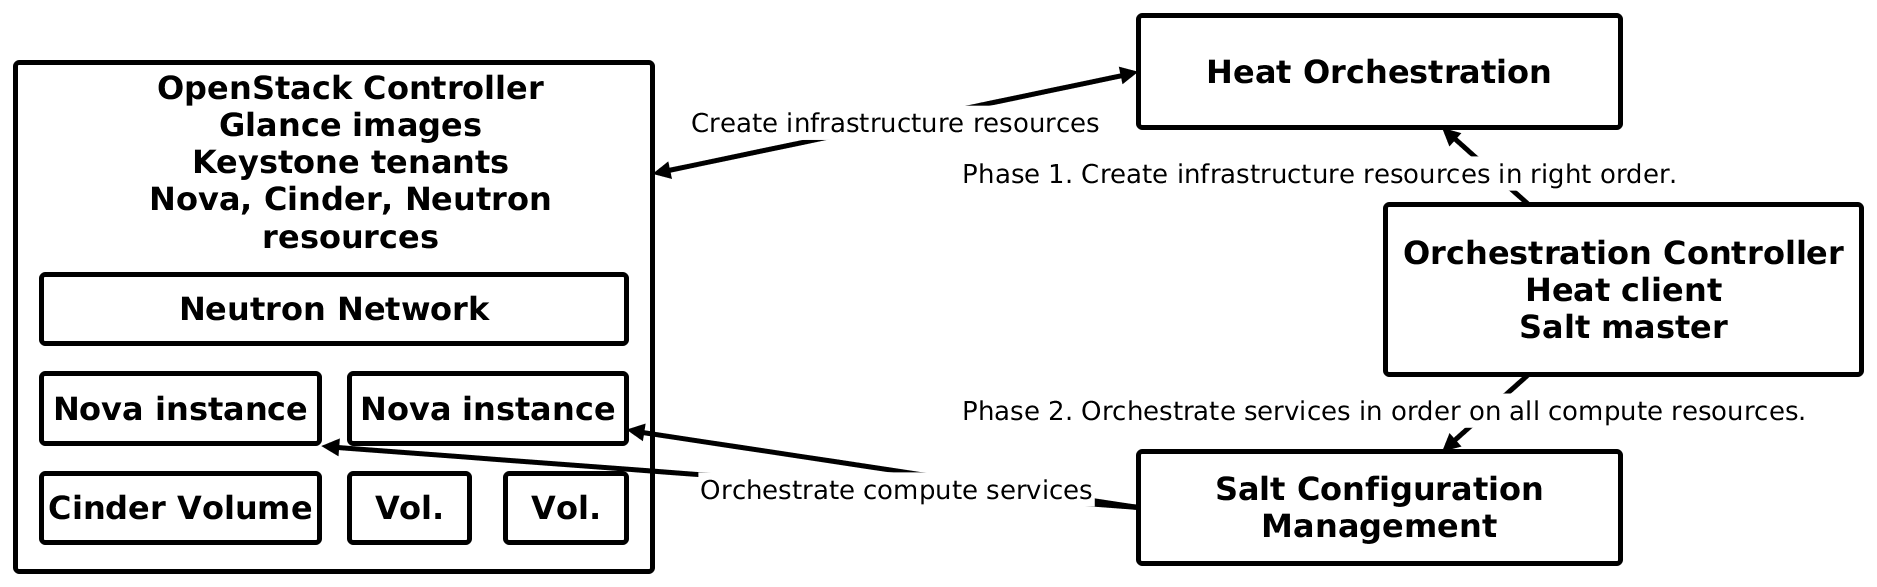
\includegraphics[scale=0.21]{images/heat}
\par\end{centering}
\caption{Popis heat orchestrace\label{fig:heat}}
\end{figure}

\section{Load balancer as a Service}

Jednou z nejčastějších síťových funkcí, která je v dnešních počítačových síťích a datových centrech vyžadována je load balancing. Load balancer spravuje příchozí komunikaci a distrubuje ji do několika serverů či jiných síťových zdrojů. Tím je zajištěna rozloha zátěže.  V cloudovém prostředí je tedy možné velice rychle, dle požadavků uživale či automaticky dle nastavených parametrů, škálovat (přidávat či odstraňovat) webové servery. Load balancer zároveň monitoruje stav jednotlivých sleduje stav jednotlivých instancí a posílá komunika pouze správně fungujícím instancím. 

Na obrázku č. \ref{fig:LoadBalancer} je vidět celý koncept load balanceru poskytovaného jako službu v privátním cloudu. Každý uživatel má možnost si dle potřeby vytvořit load balancer pro sve webové servery. Pokud provozuje několik webových služeb v jednom projektu (tenantu), může pro každou tuto službu vytvořit vlastní load balancer, který bude nakonfigurován dle požadavků. Tento load balancer je dostupný pro všechny uživatele cloudu, tedy ve všech tenantech.

\begin{figure}[h]
\begin{centering}
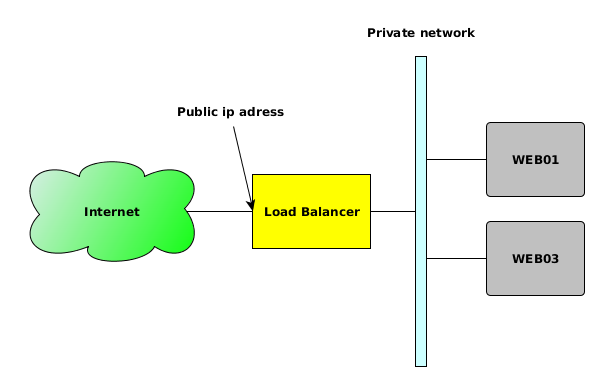
\includegraphics[scale=0.43]{images/LoadBalancer}
\par\end{centering}
\caption{Load Balancer as a Service\label{fig:LoadBalancer}}
\end{figure}

\subsection{Neutron LbaaS}

Při výběru řešení pro load balancing je nutné zvážit především výkon load balanceru. Na trhu již existuje celá řada fyzických i virtuálních produktů. Fyzická řešení nabízí větší výkon a obvykle i více funkcí. Virtuální pak větší flexibilitu v nasazení a jednodušší konfiguraci.

Avšak existuje jednotná množina funkcí, kterou uživatelé požadují a kterou většina load balancerů poskytuje. 
OpenStack Neutron navrhl LBaaS jako pokročilou službu Neutronu, která umožňuje použít jeden soubor API k využítí load balancing funkce poskytnuté celou řadou poskztovatelů.

Zjednodušeně toto umožňuje uživatelům OpenStacku přes jedno společné rozhraní ovládat několik různých řešení pro load balancing. Zároveň díky tomu odpadá nutnost seznamování se s implementací a konfigurací těchto různých řešení, která mohou být velmi specifická a odlišná.

V této práci je ukázán příklad využítí implementace load balanceru v OpenContralu, který může být přes toto api ovládán. Avšak zde ukázané řešení může být použito s jakoukoli implementací load balanceru, at už virtuláního (sofwarového) či fyzického, pokud dokáže komunikovat s OpenStack Neutron LbaaS rozhraním. Dle dokumentace OpenContrailu \cite{contrail_loadbalancer} je v něm kontrétní implementace load balanceru řešena pomocí HAProxy. HAProxy je zdarma dostupný open source software pro unix operační systémy \cite{HAProxy}. 


Load balancer se v Neutron LbaaS skládá ze 4 objektů.

\begin{itemize}
\item Pool - Označuje síťový rozsah pro webové servery
\item Virtální IP (VIP) - ip adresa, na kteru příchází komunikace
\item Member - Označuje konktétní instanci, která je členem poolu.
\item Monitor - Monitoruje stav aplikace. Pomocí HTTP, TCP či PING.
\end{itemize}

Obrázek č. \ref{fig:NeutronLbaaS} zachycuje jednotlivé závislosti mezi těmito objekty. Celý proces probíhá tak, že každý virtuální server, který je asociovaný s daným poolem z něj obdrží IP adresu. Když příjde na VIP nějaký dotaz na danou webovou aplikaci, tak je tento dotaz předán dál na jednu z těchto přiřazeným IP adres. Pokud nastane s aplikací či serverem nějaký problém, který zachytí monitor, tak load balancer ip adresu tohoto serveru přestane posílat komunikaci, dokud není vše zase v pořádku.

\begin{figure}[h]
\begin{centering}
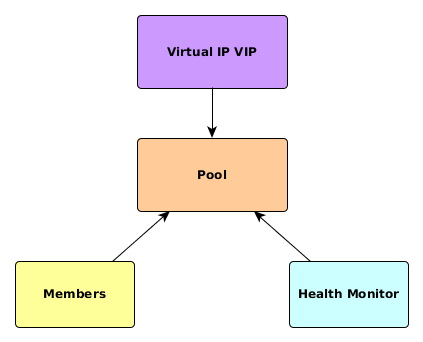
\includegraphics[scale=0.63]{images/NeutronLbaaS}
\par\end{centering}
\caption{Neutron LbaaS\label{fig:NeutronLbaaS}}
\end{figure}

\subsection{LbaaS heat template}

Aby nemusel uživatel ručně vytvářet load balancer ručně, tak byl celý proces vytváření load balanceru zautomatizovám pomocí heat templatu. Tím byla vytvořena VNF Navržený heat template pro LbaaS v sobě obsahuje následující prostředky, které se po spuštění pokusí vytvořit.

\begin{itemize}
\item pool
\item members
\item health monitoring
\item 2 web instance
\item privatni síť
\item public síť
\end{itemize}

Pro vytvoření heat stacku s Load balancerem je nutné daný template vytvořit pomocí příkazu:

\verb!heat stack-create -f heat/templates/lbaas_template.hot -e heat/env/lbaas_env.env lbaas!

Tento příkaz vytvoří všechny již uvedené prostředky pro load balancing. Konkrétní load balancer má nakonfigurovanou virtual ip adresu (VIP) a k ní přiřazenou floating adresu, která je přístupná z externích sítí. Zároveň má tento load balancer přiřazený pool, ke kterému je přiřazena přiřazena privátní síť 10.10.10.0/24. Na obrázku č. X znázorňuje tento pool a obrázek č. X+1 jsou vidět členové (members) toho poolu.

\begin{figure}[h]
\begin{centering}
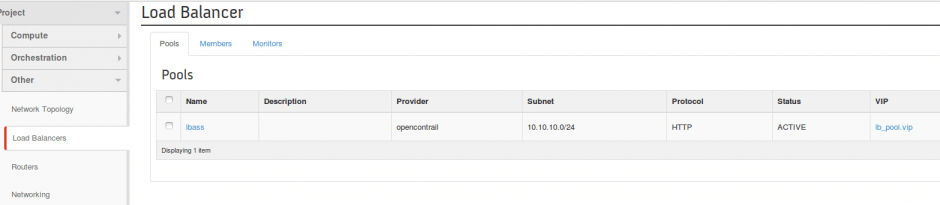
\includegraphics[scale=0.45]{images/lbaas1}
\par\end{centering}
\caption{Vytvořený pool\label{fig:lbaas1}}
\end{figure}

\begin{figure}[h]
\begin{centering}
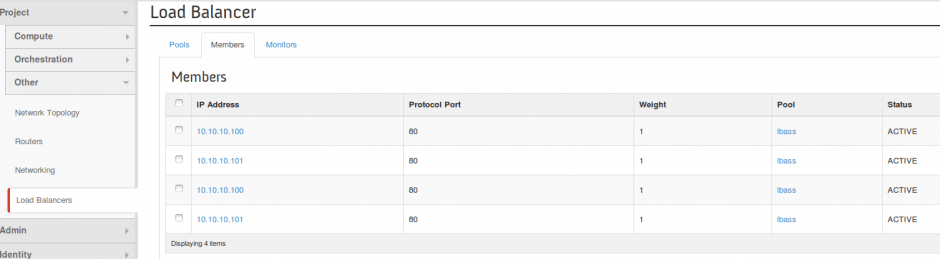
\includegraphics[scale=0.45]{images/lbaas2}
\par\end{centering}
\caption{Vytvoření members\label{fig:lbaas2}}
\end{figure}

Další zdrojem, který byl vytvořen je health monitor, který lze viděn na obrázku č. X+2. Díky němu má load balancer přehled o aktuálním stavu webových instancí. Pokud by náhodou některá z nich přestala odpovídat, v tomto případě na ping, tak by load balancer na tuto instanci přestal zasílat traffic.

\begin{figure}[h]
\begin{centering}
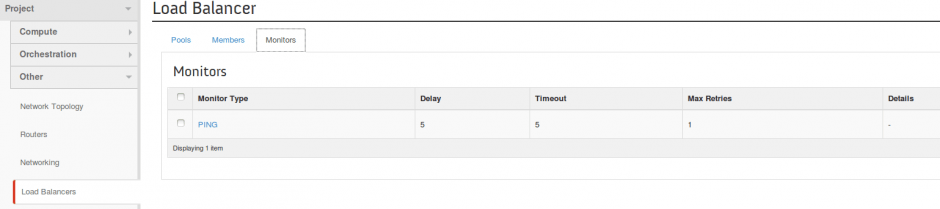
\includegraphics[scale=0.45]{images/lbaas3}
\par\end{centering}
\caption{Vytvořený health monitor\label{fig:lbaas3}}
\end{figure}

Finální síťovou topologii znázorňuje obrázek č. X+3. 


\begin{figure}[h]
\begin{centering}
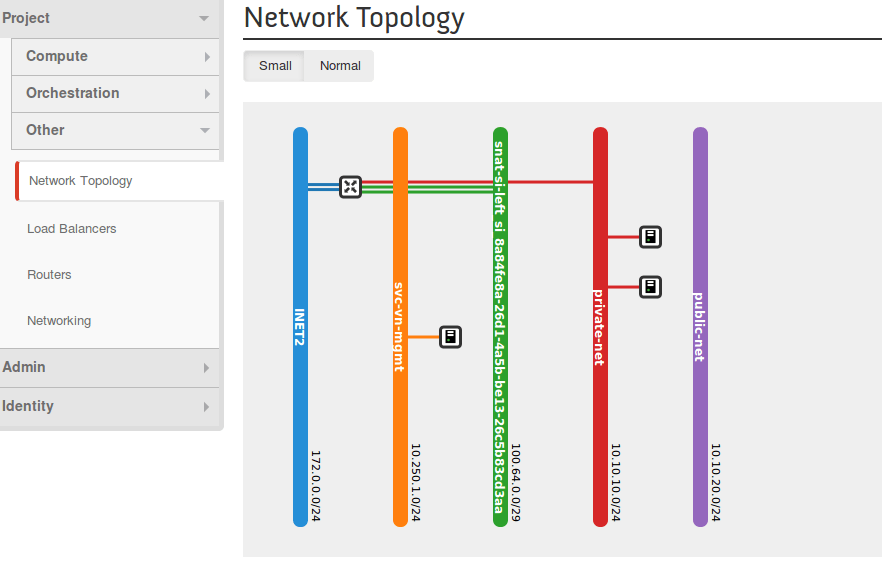
\includegraphics[scale=0.45]{images/lbaas_topologie}
\par\end{centering}
\caption{Vytvořená síťová topologie\label{fig:lbaas_topologie}}
\end{figure}

Otestování webových serverů lze provést příkazem curl, kterému dáme jako paramert ip VIP nebo floating ip load balanceru. Po několika takovýchto zadání tohoto příkazu je vidět, že oba web servery odpovídají a je probíhá mezi nimi load balancing metodou round robin.  Celý tento test je vidět na obr. č. X+4

\begin{figure}[h]
\begin{centering}
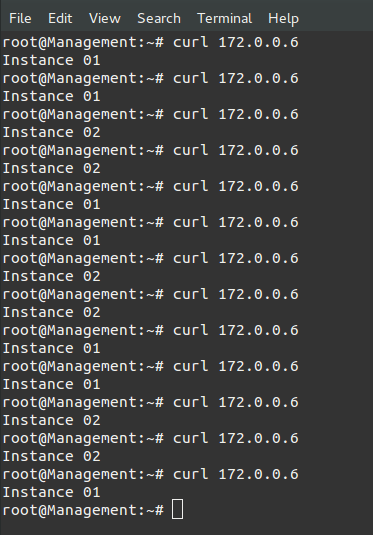
\includegraphics[scale=0.45]{images/lbaas_testing}
\par\end{centering}
\caption{Test konektivity a load balancingu\label{fig:lbaas_testing}}
\end{figure}




\section{Firewall as a Service}

Servisní Template obsahuje obecný předpis pro danou VNF. Mezi tyto informace patří:

\begin{itemize}
\item Název - Název je označení daného Servisního Templatu. Pomocí něho lze následně identifikovat daný template a spustit dle jeho parametrů Servisní instanci. 
\item Image - Image je image, který má být použit pro vytvoření dané servisní instance. V našem případě se bude jednat o image, který obsahuje požadované síťové funkce. Tento image musí před tím než může být použit  nahrán do OpenStacku přes glance.
\item Service Type - V OpenContrailu, prozatím existují dva typy. Jsou to Trafic Analyzer a Firewall. Pro účely této práce bude používán pouze typ Firewall.
\item Service Mode - Zde se určuje v jakém modu daný template bude nastaven. Jsou zde možnosti In-Network, In-Network-NAT.

\item Typy síťových portů - Zde se určuje kolik portů bude daná instance, vytvořená pomocí tohoto templatu mít a jaká bude jejich role. Jsou zde možnosti Left, Right a Management. 

\end{itemize}

Po uspěšném vytvoření Servisního templatu je možné z něj vytvořit libovolný počet Servis Instancí. Ty běží jako klasické instance v OpenStacku, avšak OpenContrail s nimi zachází jiným způsobem. 

\begin{itemize}
\item 1 firewall instanci
\item 1 testovaci instanci
\item 1 management instanci
\item management síť
\item privátní síť
\item contrail policy
\end{itemize}

\subsection{Scénář NAT}


\begin{figure}[h]
\begin{centering}
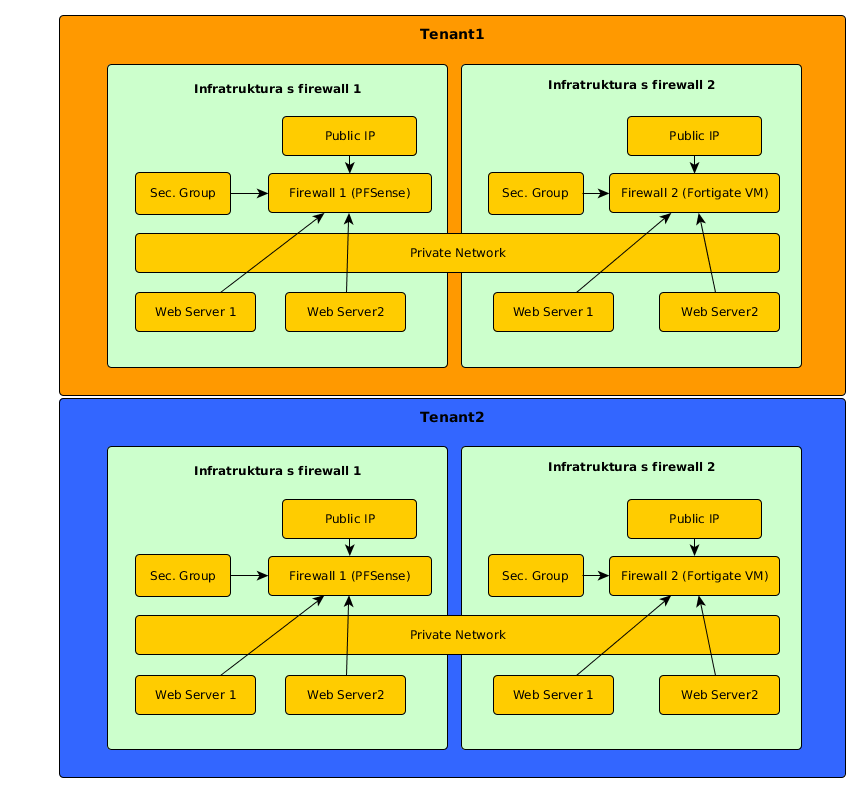
\includegraphics[scale=0.43]{images/firewall}
\par\end{centering}
\caption{Firewall as a Service\label{fig:firewall}}
\end{figure}

\subsection{Scénář HA firewall}

\begin{figure}[h]
\begin{centering}
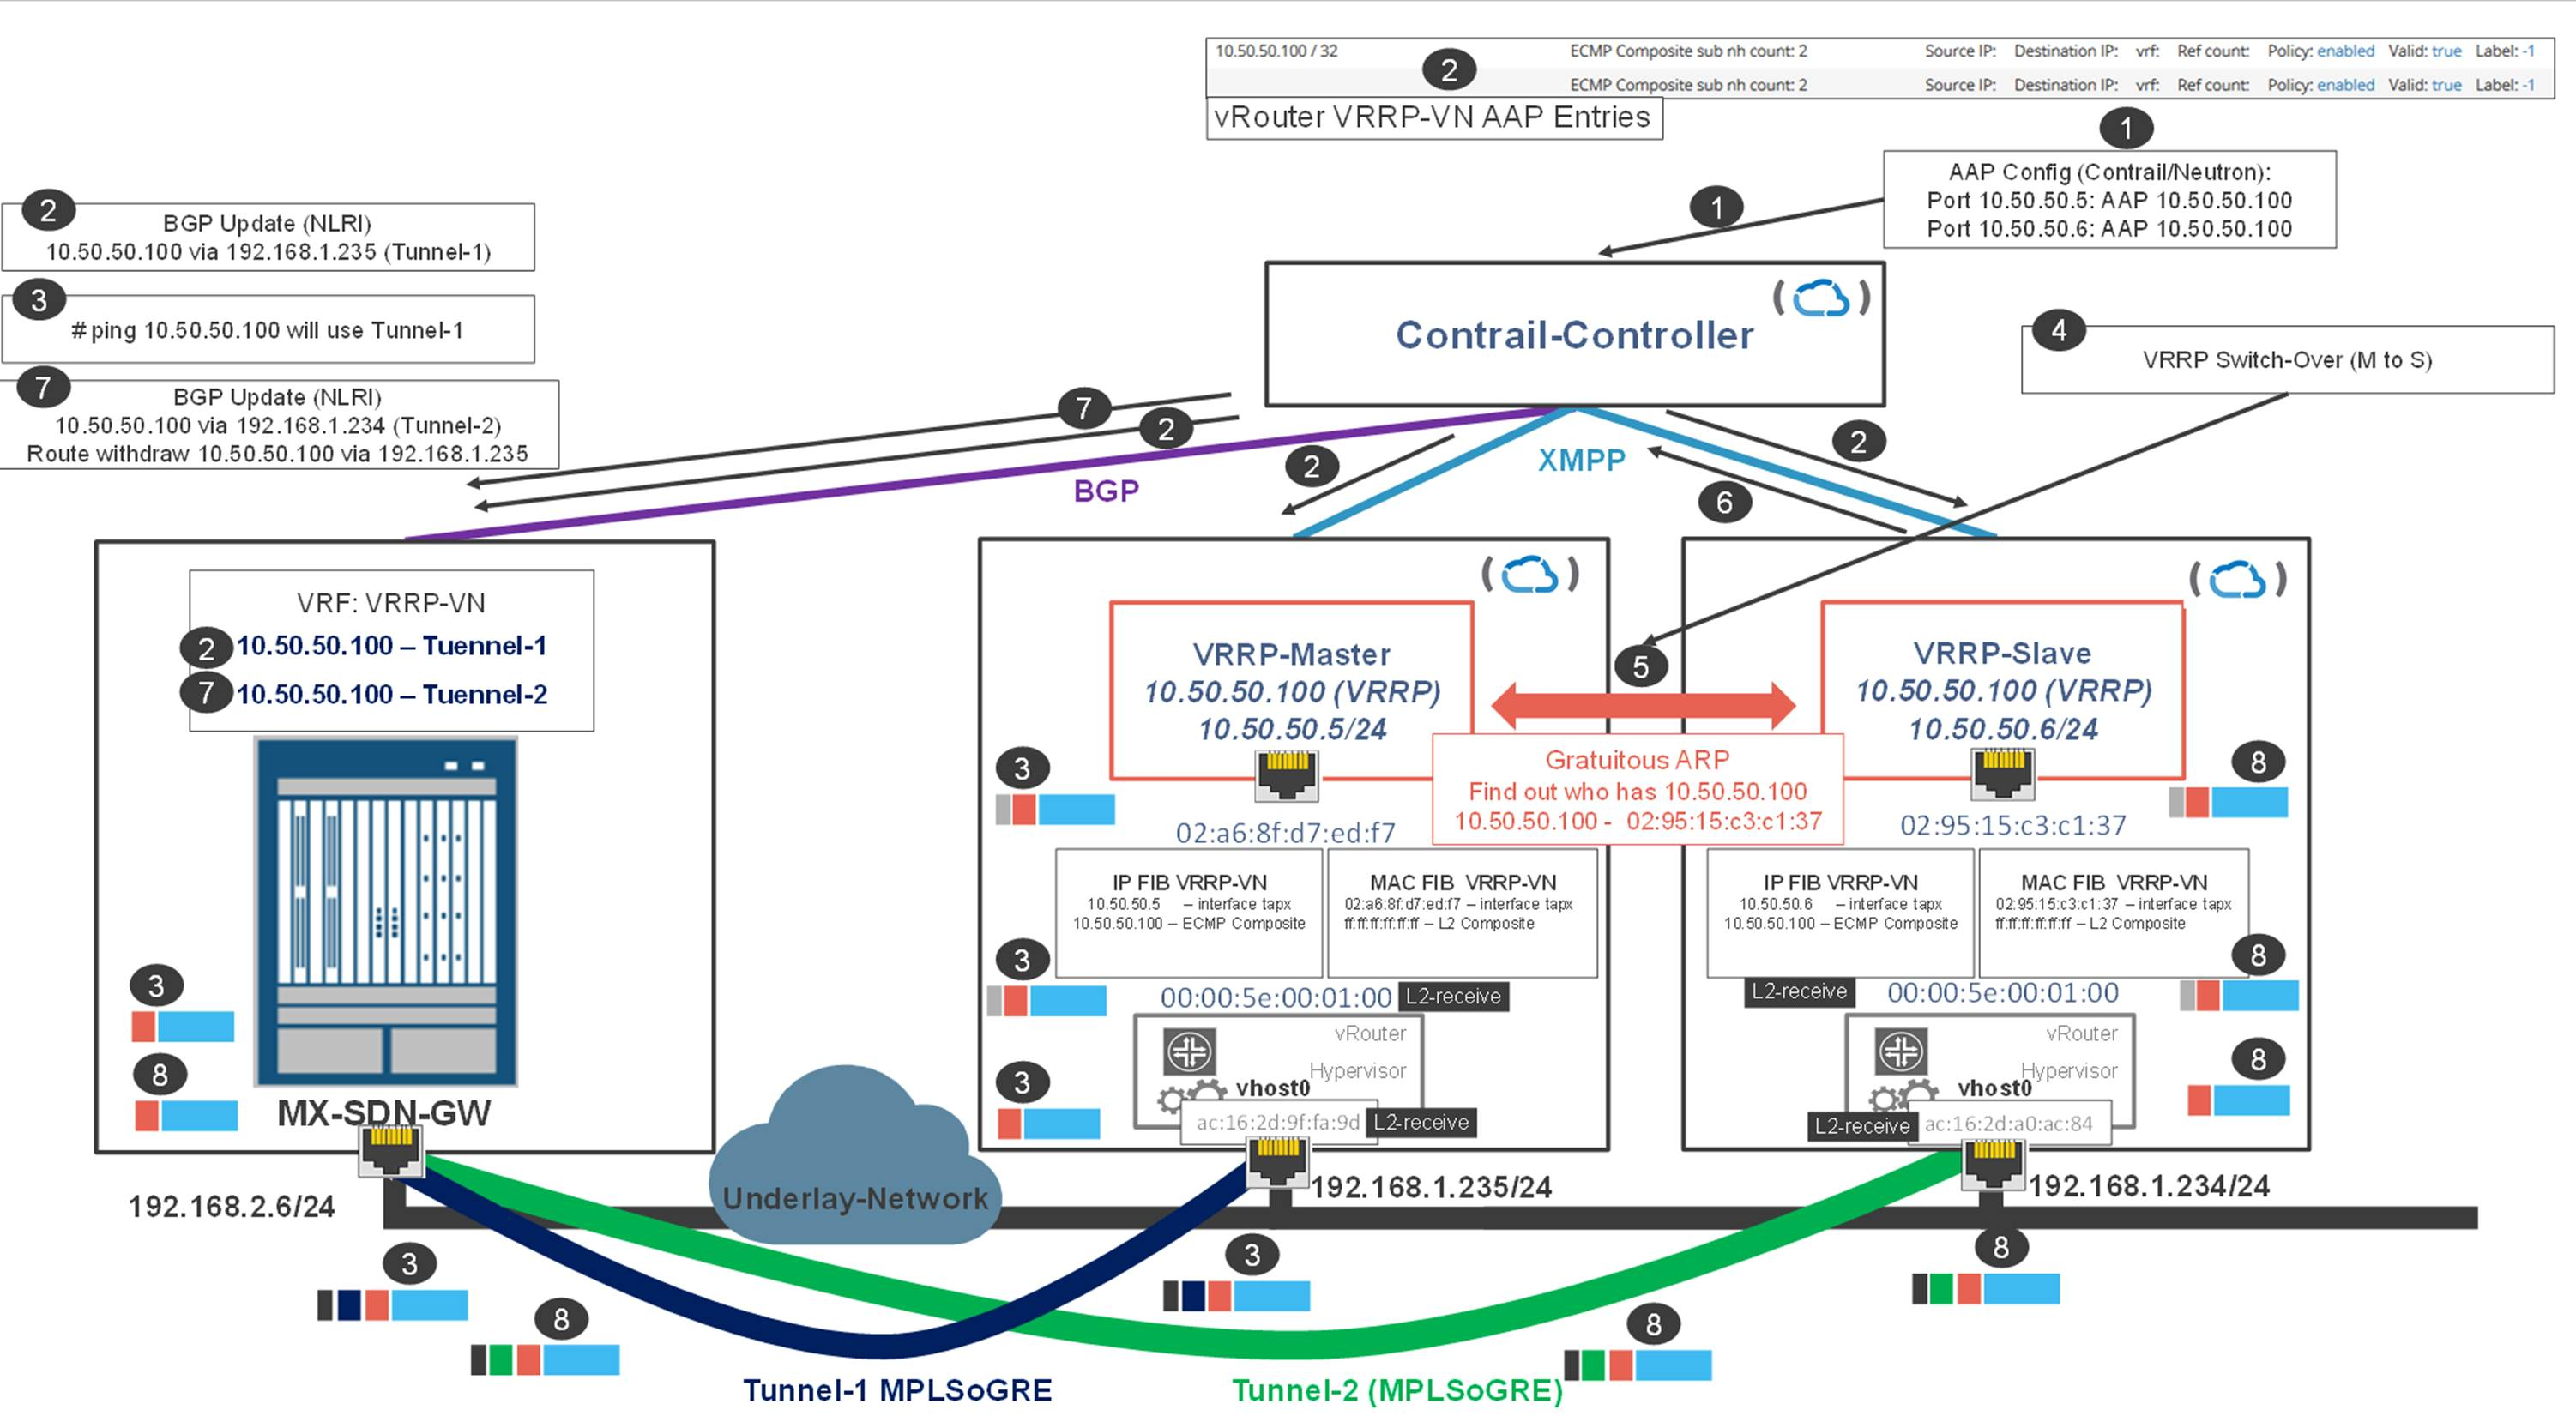
\includegraphics[scale=0.11]{images/contrailHA}
\par\end{centering}
\caption{High Availability Firewall\label{fig:contrailHA}}
\end{figure}


\subsection{FwaaS template}

Pro FwaaS je narhnut heat template, který obsahuje:





